In modern research in particles physics one approach of data acquisition is the collisions of acclerated particles, which interact during the collision via the known \acs{SM} interaction described in section \ref{sec:section_1_1} or possible unknown \acs{BSM} interactions. The products of interaction between can then be detected by analyzed by physicists. \\

In this thesis the data, which is analyzed for the search of \acs{LFV} in Z boson decays, is produced by proton-proton-collisions, of the Large Hadron Collider (\acs{LHC}) \cite{LHC} and detected by the Compact Muon Solenoid (\acs{CMS}) \cite{CMS} in the year of 2016. Both apparatus are explained in the following sections, proton physics is explained in section \ref{sec:section_2_1_2}.


\section{Large Hadron Collider}
\label{sec:section_2_1}

The \acs{LHC} is a circular proton-proton-collider with a center of mass energy of $\sqrt{s} = 13$ tera electron volt (\acs{TeV}) \cite{LHC2}, which is located at the European Organization for Nuclear Research (\acs{CERN}) in Geneva. The accleration of the protons is done by a system and of pre-accelerators, which feeds the protons then in the LHC to reach the designed center of mass energy, see figure \ref{fig:fig_2_1} for a schematic overview. \\

\begin{figure}[ht]
	\centering
	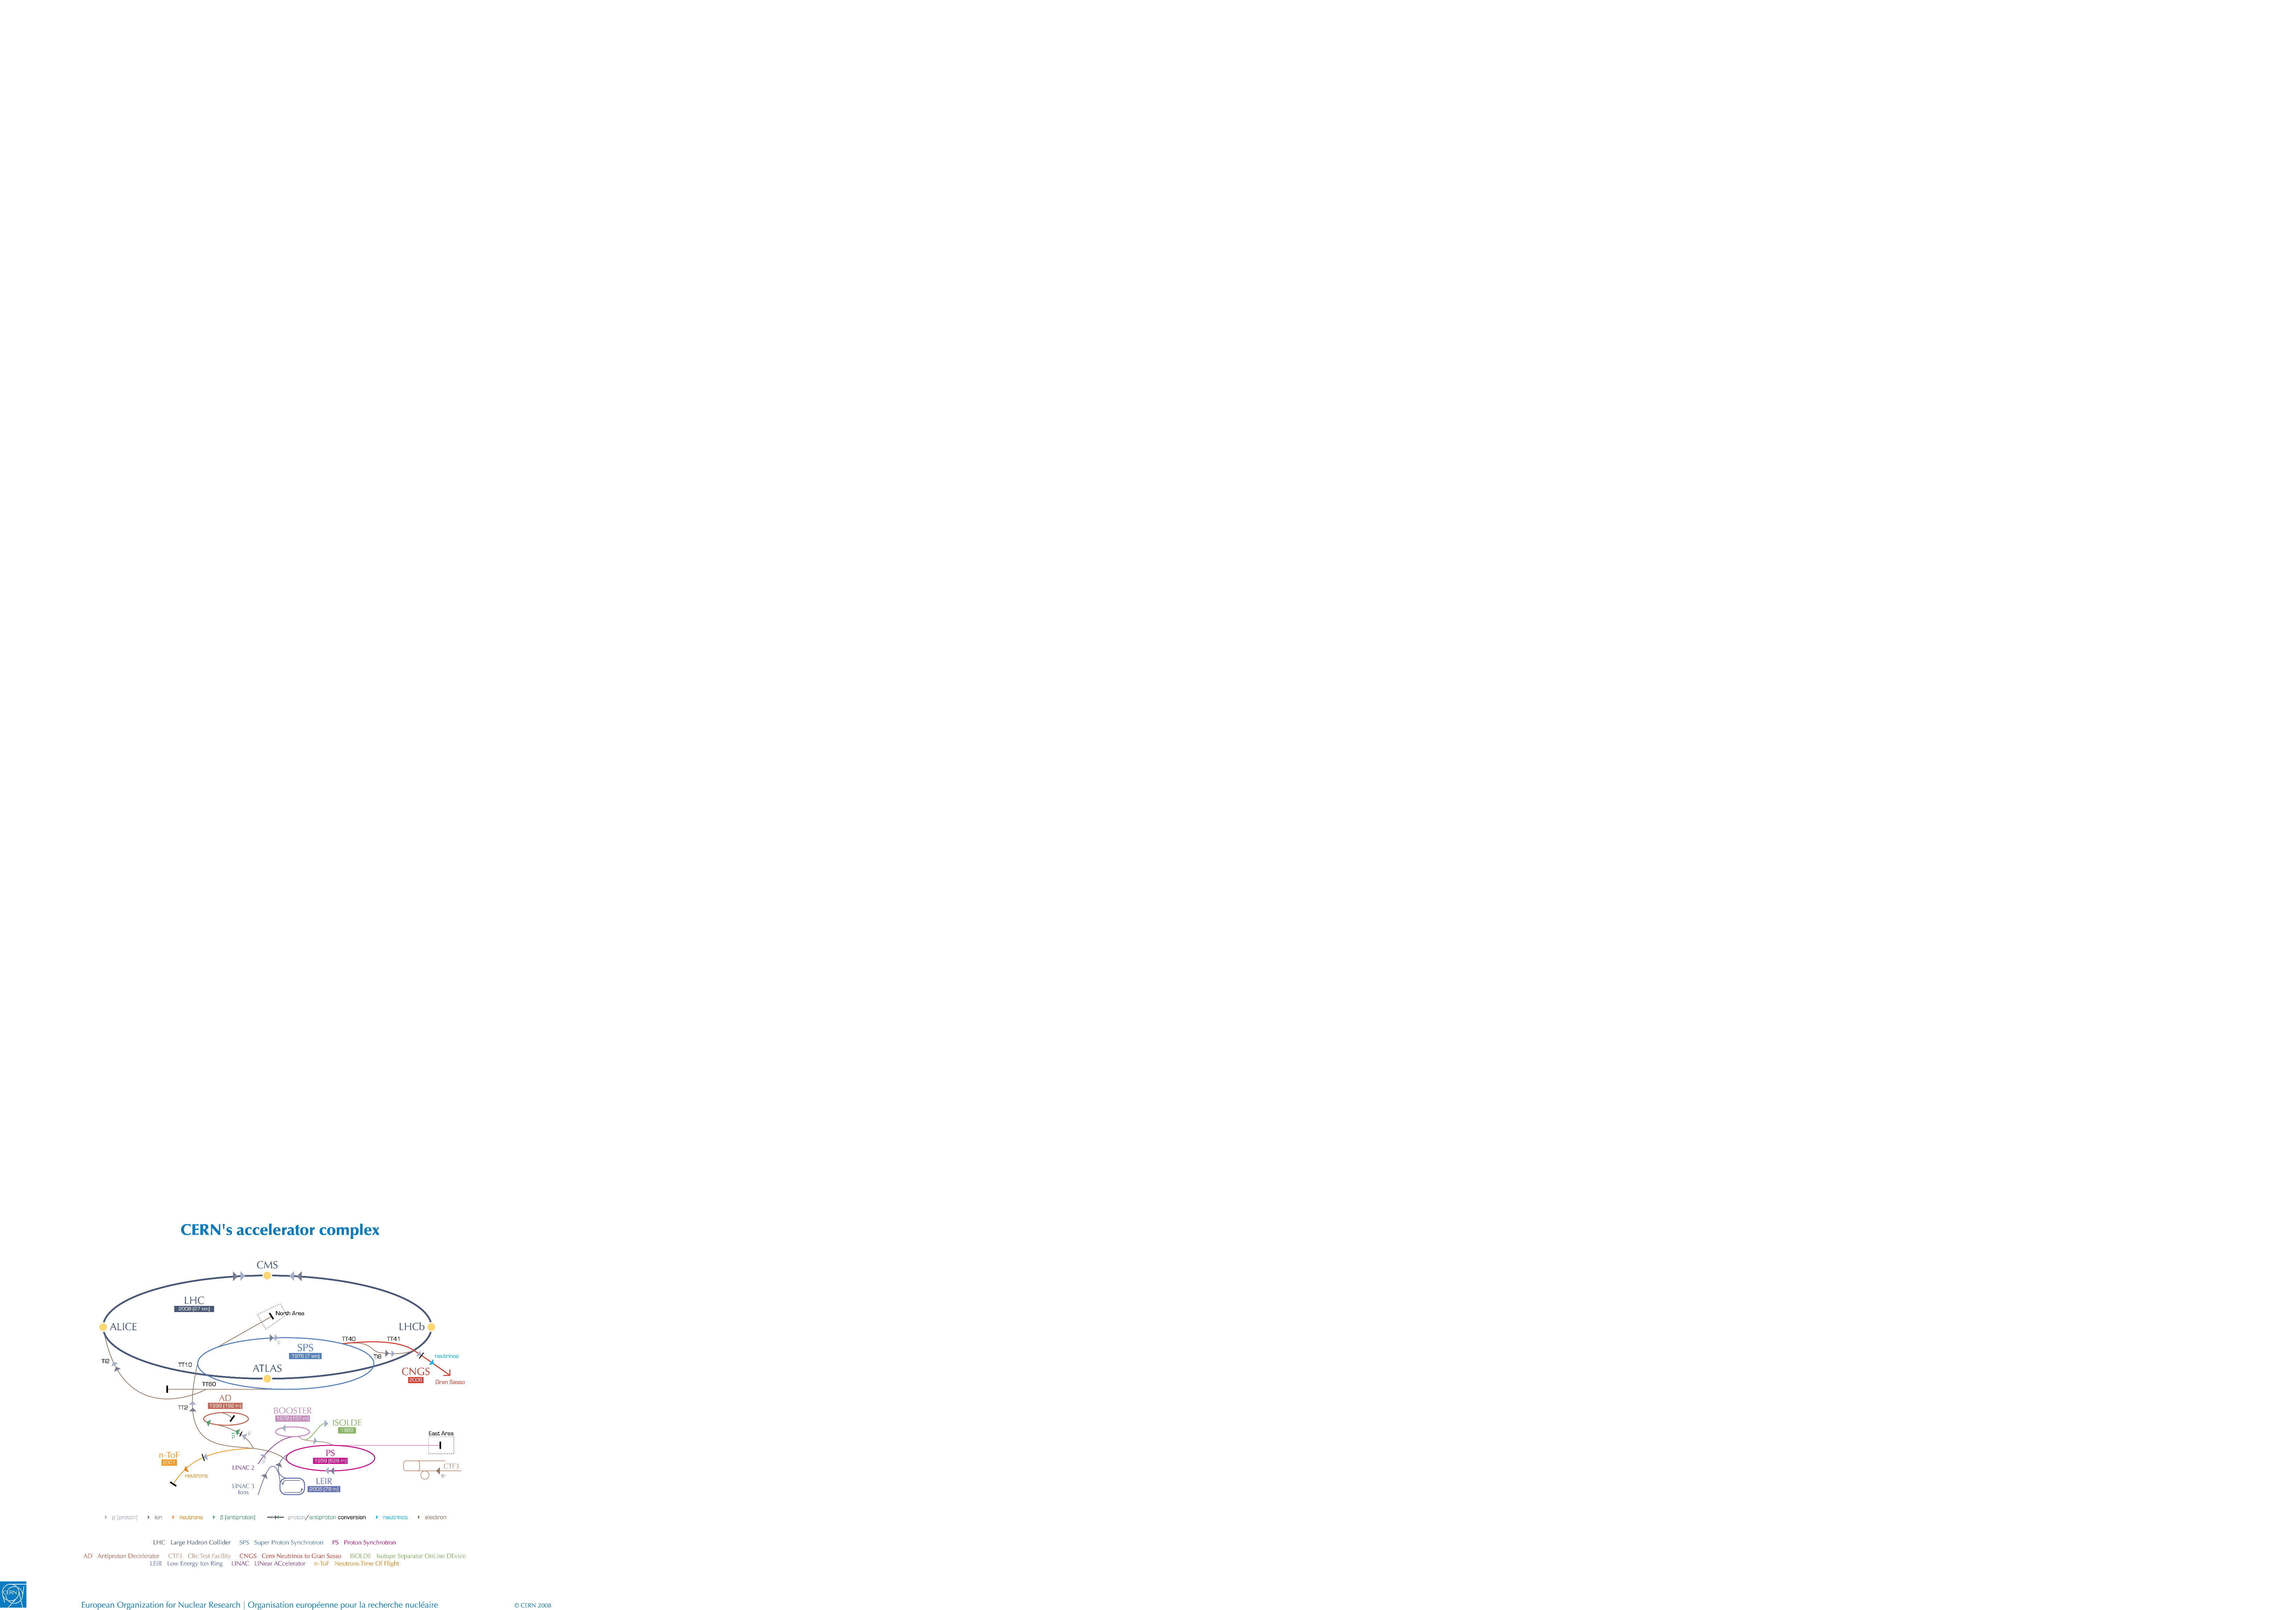
\includegraphics[width=1.0\textwidth]{pictures/LHC.pdf}

	\caption[Schematic overview of CERN accelerator complex]{Schematic overview of \acs{CERN} accelerator complex, including the \acs{LHC} and the previous pre-acclerators. The yellow points mark the position of the particles detectors at the collisions points. Taken from \cite{LHCACCL}}
	\label{fig:fig_2_1}
\end{figure}

At each collision point of the proton beams a sophisticated detector system is installed, indicated by the yellow dots in figure \ref{fig:fig_2_1}. Each of this detectors is designed for a special purpose of particle detection. The four big experiments are the \acs{CMS} and A Toroidal LHC Apparatus (\acs{ATLAS}) \cite{ATLAS}, which are designed to probe \acs{SM} and \acs{BSM} physics, the Large Hadron Collider beauty (\acs{LHCb}) \cite{LHCb}, which is designed for decays of hadrons, and the A Large Ion Collider Experiment (\acs{ALICE}) \cite{ALICE}, which is designed for heavy ion collisions.


\subsection{Properties of the proton beams}
\label{sec:section_2_1_1}

The protons in the \acs{LHC} are accelerated in so-called bunches, which contain around $10^{11}$ protons, and are seperated in space by a time interval of 25 ns \cite{LHCSTATS}. The size of the bunches is oscillating due to dynamics of the charged protons in the magnetic system of the \acs{LHC} \cite{LHC} and the beam size can be parametrized by the emittance $\epsilon$, which describe the cross section of the beam, and the $\beta$ function, which describes the oscillation amplitude \cite{BEAMPHY}. The properties of the beams has a high impact on the quality on the collider, which is parametrized by instantaneous luminosity $\mathcal{L}$ \cite{Luminosity}

\begin{equation}
	\label{eq:eq_2_1}
	\mathcal{L} = \frac{\gamma \cdot f \cdot k_{b} \cdot n_{1} \cdot n_{2}}{4 \cdot \pi \cdot \epsilon \cdot \beta}
\end{equation} 

with Lorentz gamma factor $\gamma$, the revolution frequency $f$ of the bunches, the number of colliding bunches $k_{b}$ and the number of protons $n_{i}$ in each bunch. Because the information about the properties are incoded in the luminosity, there is a direct dependence of rate $\frac{dN}{dt}$ of collisions events to the luminosity, and the total number $N$ of collisions events to the integrated luminosity $\mathcal{L}_{int}$

\begin{equation}
	\label{eq_2_2}
	\begin{split}
		\frac{dN}{dt} = \sigma \cdot \mathcal{L} \\
		N = \sigma \cdot \mathcal{L}_{int}
	\end{split}
\end{equation}	

with $\sigma$ as the cross section of proton-proton collisions. So the beam parameter have a direct influence on the total number of possible recorded events and the amount statistics which is provided for the analysis. Figure \ref{fig:fig_2_2} shows collected integrated luminosity of the data-taking run in 2016 in dependence of the day. 

\begin{figure}[ht]
	\centering
	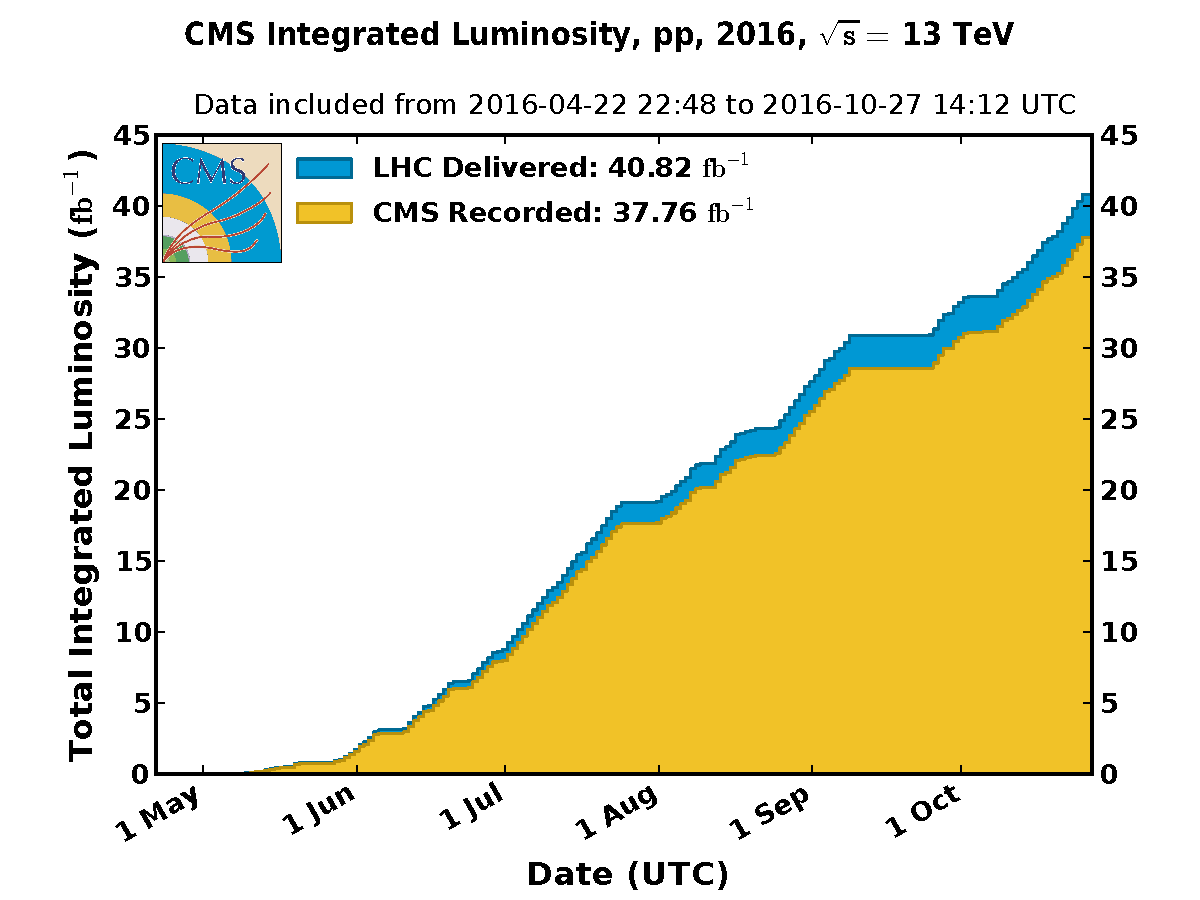
\includegraphics[width=0.7\textwidth]{pictures/int_lumi_per_day_cumulative_pp_2016.pdf}

	\caption[Total integrated luminosity of the year 2016]{Total integrated luminosity collected by \acs{CMS} in the run in the year 2016, taken from \cite{CMSLUMI}}
	\label{fig:fig_2_2}
\end{figure}


\subsection{Proton-proton collisions}
\label{sec:section_2_1_2}

Protons are non-elementary hadrons, which are a bound state of three quarks, in this case of two up-quarks and one down-quark. This bound state can be described by \acs{QCD}, see section \ref{sec:section_1_1_2}, and give rise to the quark-parton model \cite{Peskin}. In this description protons composite of the so-called partons, which are beside the three quarks of the bound state, other quarks and gluons which are produced/annihilated during the interaction in the bound state. Each of the quarks and gluons carry a fraction $x$ of the total momentum $P$ of the proton, and the probability of a existing parton with flavour f, with $f \in (u, d, \bar{u}, \bar{d}, ... g)$ and with $x$ is described by the parton density function (\acs{PDF}) $f_{f}(x)$ \cite{Peskin, PDF1}. \acsp{PDF} are not predictable by \acs{QCD} and have to be measured in deep inelastic scattering processes, figure \ref{fig:fig_2_3} shows the measurement of the \acsp{PDF} in the ZEUS experiment \cite{ZEUS}. \\

\begin{figure}[ht]
	\centering
	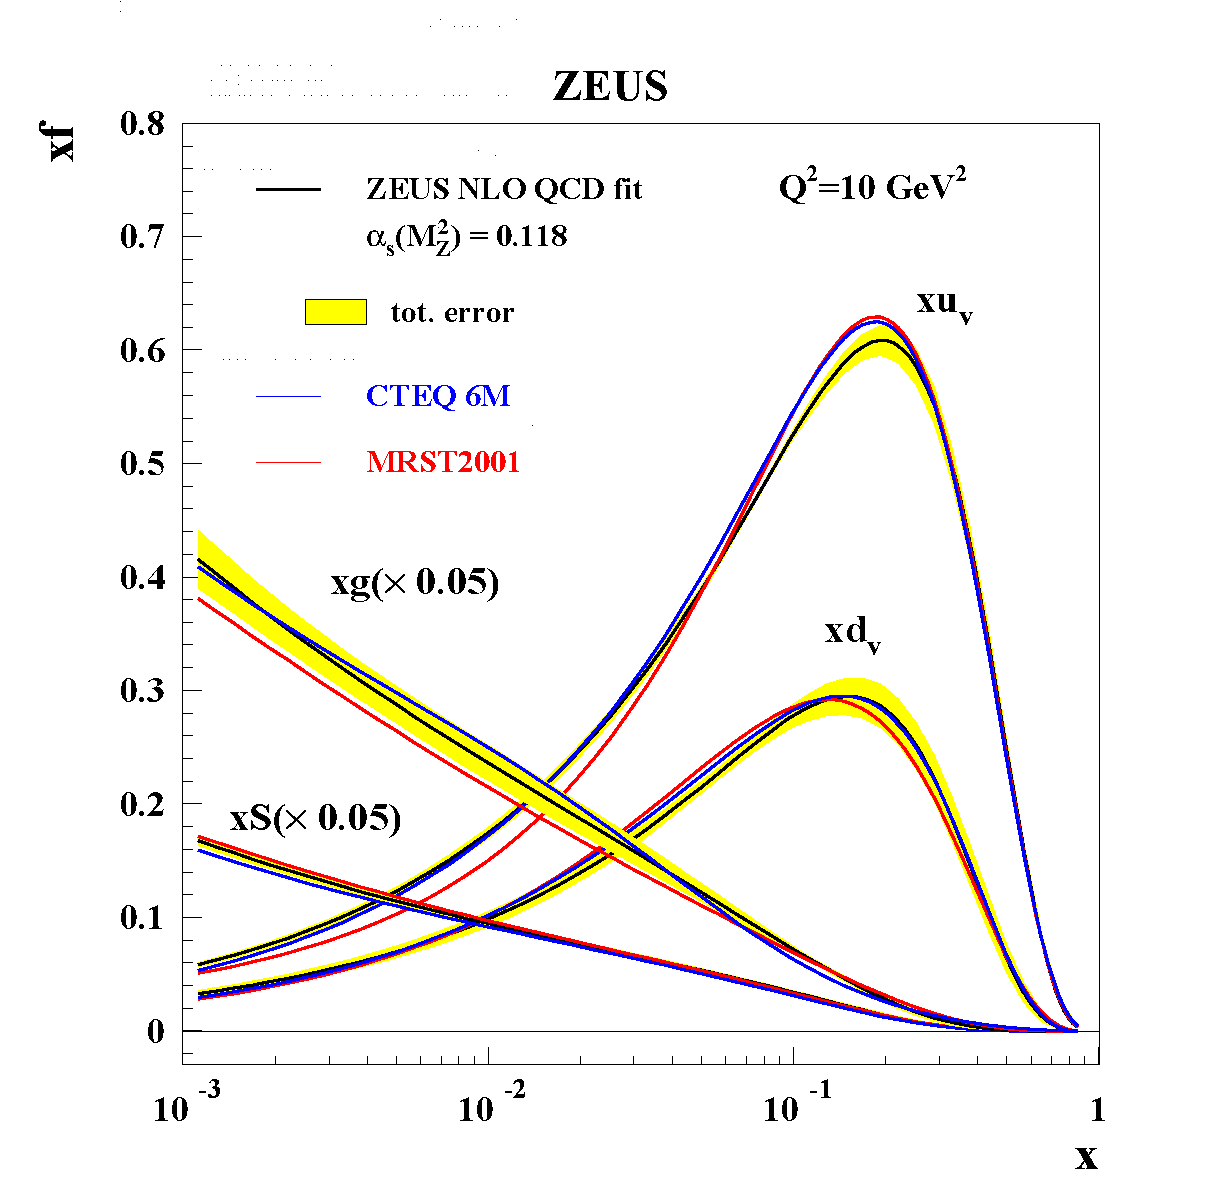
\includegraphics[width=0.7\textwidth]{pictures/ZEUS_PDF.pdf}

	\caption[Proton \acsp{PDF} from ZEUS]{\acsp{PDF} of up-quarks, down-quarks and gluons in a proton measured by the ZEUS experiment, taken from \cite{PDFMEAS}}
	\label{fig:fig_2_3}
\end{figure}

In collisions of the protons at the \acs{LHC} the interaction depens on the \acsp{PDF} and the $x_{i}$ of the partons. Taking as example proton-proton collisions into fermion pair production, two quarks with momentum $x_{1}P$ and $x_{2}P$ will produce the fermion pair, all the other constituent $X$ are not partizipating in the interaction and carry away the remaining proton momenta, see figure \ref{fig:fig_2_4} for a schematic example. The cross section $\sigma(pp\to f\bar{f} + X)$ \cite{Peskin} for such a process in the dependence on the $x_{i}$ and the \acsp{PDF} is 

\begin{equation}
	\label{eq:eq_2_3}
	\int_{0}^{1}dx_{1}\int_{0}^{1}dx_{2}\sum_{f \in (u, d, \bar{u}, \bar{d}, ... g)} f_{f}(x_{1})f_{\bar{f}}(x_{2}) \cdot \sigma(q_{f}(x_{1})q_{\bar{f}}(x_{2}) \to f\bar{f}) 
\end{equation}


\begin{figure}[ht]
	\centering
	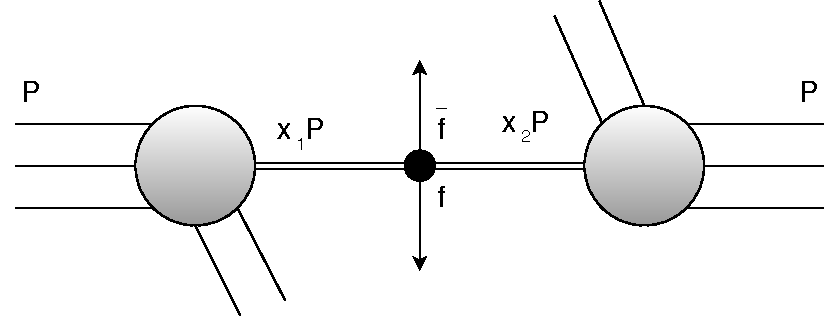
\includegraphics[width=0.7\textwidth]{pictures/ppcollision.pdf}

	\caption[Schematic sketch of proton-proton collision]{Schematic sketch of a proton-proton collision at the \acs{LHC}. The protons have momentum $P$, the quarks involved in the interaction have the fraction $x_{i}$ of it, all other rest carries away the remaining momenta}
	\label{fig:fig_2_4}
\end{figure}


\section{Compact Muon Solenoid}
\label{sec:section_2_2}


\begin{figure}[ht]
	\centering
	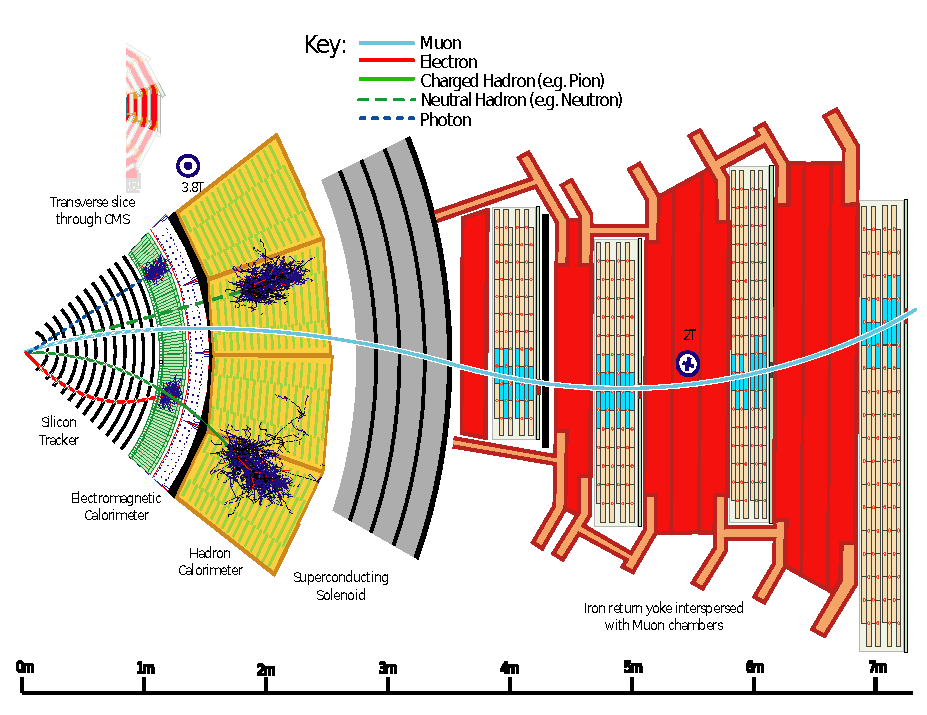
\includegraphics[width=0.7\textwidth]{pictures/CMS.pdf}

	\caption[Profile of CMS detector]{Schematic sketch of the profile of \acs{CMS} with detectors and possible particle and their interactions in the detectors, taken from \cite{PARTICLEFLOW}}
	\label{fig:fig_2_5}
\end{figure}

